\section{\heiti{理论及算法}}

\subsection{\heiti{离散傅立叶变换(Discrete Fourier Transformatioin, FFT) 的快速实现}}

基于第二部分经典理论,本项目实现高精度 FFT 流处理器的主要方式如下所述。
\paragraph{\heiti{高性能 FFT 流处理器:基于冗余计算和折叠架构的浮点运算蝶形阵列}}
为实现小面积、高并行、高灵活度的 FFT 处理单元,本文创新性地提出了FFT流处理器,通过冗余计算和架构折叠来取得面积和运算效率的最佳权衡。

该部分创新点可总结为:
\begin{itemize}
    \item   基于冗余计算提出了具有极短关键路径的``冗余串行乘法''单元和``冗余浮点加法单元'',
    他们的关键路径仅有 $2$ 到 $3$ 个全加器(Full Adder,FA)。
    \item   通过乘加运算折叠(Folding)使得浮点数运算的复杂度极限接近定点数运算。
    \item   通过蝶形单元展开(Unfolding)使得选用各层同性FFT拓扑成为可能,从而充分简化系统控制逻辑,减少硬件运算单元在处理数据中的等待和空拍,提高硬件资源利用率。
    \item   依赖于数据的冗余表示法和各层同性的 FFT 拓扑,实现了紧凑的数据流映射方案。
    \item   使得系统的面积效率获得较大提升。
    \item   具体而言:(1)通过折叠乘加运算;(2)通过扩大蝶形单元并行度。
\end{itemize}

总结而言,在设计策略上,本文通过冗余计算使得浮点数乘、加运算取得较好的架构折叠方案;进一步通过灵活应用折叠和展开技术,实现了在相同面积约束下
,乘、加子运算并行度与蝶形单元个数(FFT处理点数并行度)之间的权衡,从而取得较为理想的面积效率。

此外更加高效的办法是参考 \cite{Li2010}。或者关于快速傅立叶变换的综述性质书籍\cite{Nussbaumer1982}。

\paragraph{\heiti{基于冗余计算的折叠蝶形计算阵列}}
图\ref{fig:Float-Redundant-Butterfly-Unit} 所示 Butterfly Unit 完成 FFT 所需的蝶形运算即
\begin{eqnarray*}
    \left\{
        \begin{aligned}
        E=Y+R\cdot X\\
        F=Y-R\cdot X
        \end{aligned}
        \right.
\end{eqnarray*}

而完成一个蝶形运算共需要两级流水线:
\begin{itemize}
    \item \heiti{第一级流水线}为冗余乘法:FFT上一级蝶形运算的输出,
            经过 Mapping 拓扑映射单元送往当前蝶形运算的输入端,
            随着输入数据的串入,乘法执行结束,与次同时,
            乘法器的输出也逐个数位地输入到 Aligning Buffer 中,
            便于后续冗余加、减法操作;
    \item \heiti{第二级流水线}为冗余浮点加、减法:
            从 Aligning Buffer 先后输出的数据被加、减归约,
            其输出被送往 Mapping 单元,以便输送给 FFT 下一级蝶形运算对应蝶形结的输入端。
\end{itemize}


\begin{center}
    \begin{figure}[ht!]
        \centering
        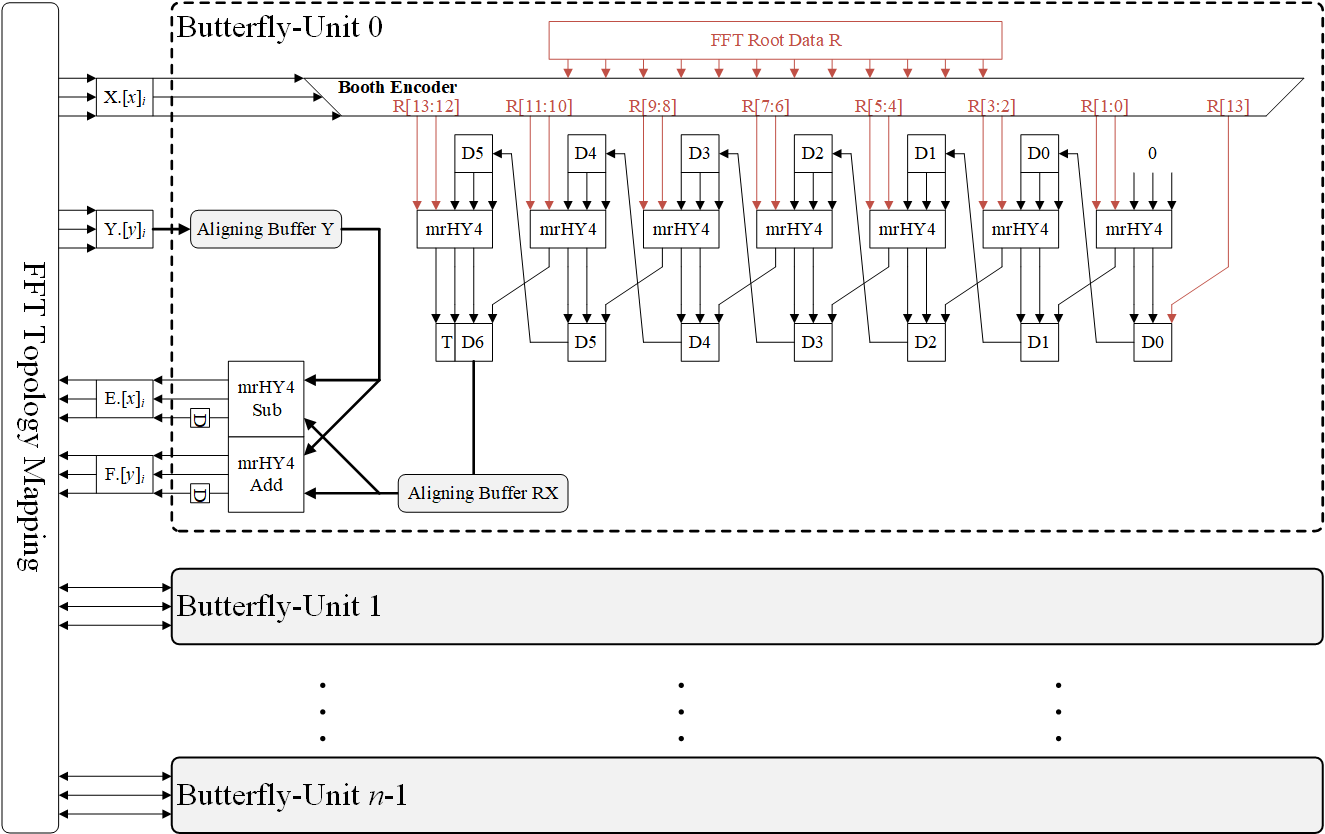
\includegraphics[width=0.6\textwidth]{figures/Float_Redundant_Butterfly_Unit.png}
        \caption{蝶形运算单元}
        \label{fig:Float-Redundant-Butterfly-Unit}
    \end{figure}
\end{center}

在这一过程中,两级运算流水执行,并无空闲等待时间,如下图任务流程图所示。
每级流水的执行时间与量化精度(即冗余量化位 $LEN$)有关,且乘法与加、减法所需执行周期均等于量化位数 $\mathrm{LEN}$。
对于一个$N=2^n$ 点的FFT,其共包含 $\log_2N$ 级别蝶形运算,故而系统工作的总周期数为:
\begin{equation*}
    (\log_2 N+1)\cdot \mathrm{LEN},\qquad \tag{C1}
\end{equation*}

Mapping 模块实现了如下图所示拓扑。得益于选用折叠的乘法和加法结构,
每个蝶形计算单元的面积已经尽可能地减小了,故而降低了多点数全并行蝶形单元的部署压力。
\begin{center}
    \begin{figure}[h!]
        \centering
        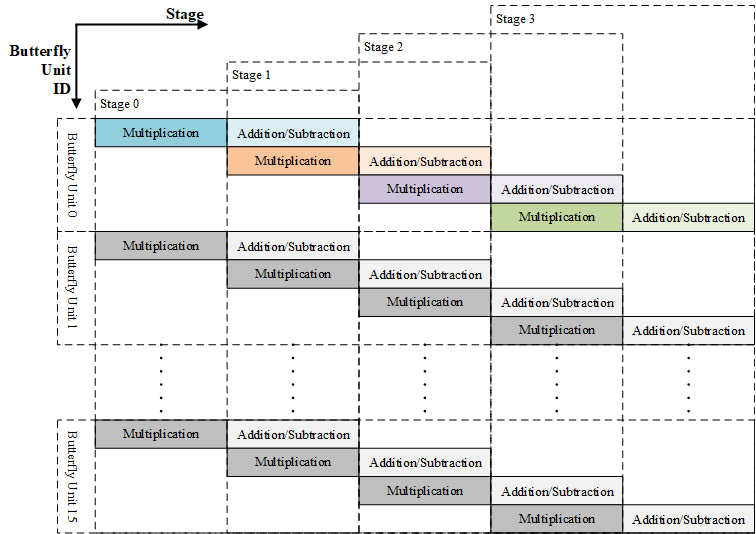
\includegraphics[width=0.5\textwidth]{figures/Pipeline.png}
        \caption{项目流水线示意图}
        \label{fig:Pipeline}
    \end{figure}
\end{center}

在我们的处理模块中,$N$ 个蝶形单元并行处理数据,它们的输出经过 Mapping 模块映射到其他蝶形单元的输入端,
结合流水化的运算流程,全自动地完成FFT的多级计算,
除了原根输入和 Reset 操作外,整个系统不包含状态机和控制逻辑,实现了自动化的流处理操作。

\subsection{\heiti{Booth 无进位乘法和 Karatsuba 快乘(Booth Multiplication Algorithms \& Karatsuba Multiplication)}}

本文选用了``基四最小冗余(Minimal Redundant Radix-4,mr4)''方案,
对于任意一个 $2n$ 二进制位的整数 $X\in\Z$,其mr4冗余表达式为:
\begin{eqnarray*}
    X=\sum_{i=0}^{n-1}[x]_i\cdot 4^i
\end{eqnarray*}

其中数位 $[x]_i\in\{-2,-1,0,1,2\}$,在计算机中 $[x]_i$ 由三个比特 $\{x_i^{-2},x_i^{+},x_i^{++}\}\in\{0,1\}^3$ 表示,即
\begin{eqnarray*}
    [x]_i=-2\cdot x_i^{-2}+x_i^{+}+x_i^{++}
\end{eqnarray*}

相较于传统的二进制补码表示法,mr4冗余表示具有以下三点优势:
\begin{itemize}
    \item   传统的存在进位传播的二进制加法在硬件实现时往往要考虑进位传播;
            而冗余示数法具有多映射的特点,即相同的 $X$ 具有多个不同的冗余表达式,
            利用这一特点,我们可以实现无``进位传播''的冗余加法,如图``基四最小冗余混合加法(mrHY4A)'',如下图\ref{fig:mrHY4A}。
            \begin{center}
                \begin{figure}[ht!]
                    \centering
                    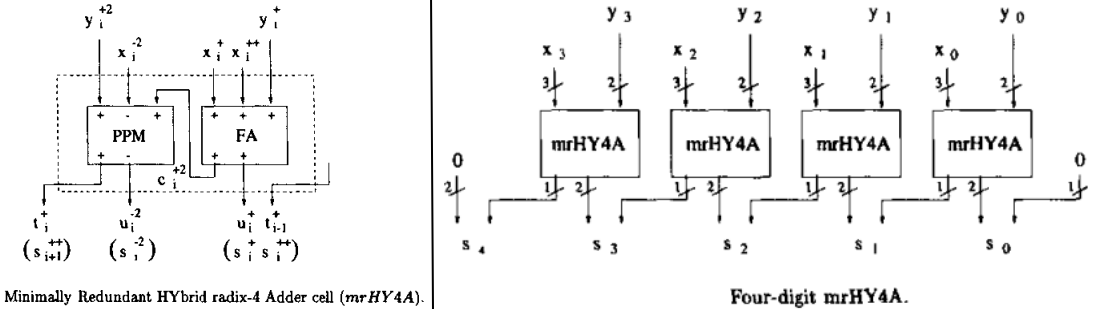
\includegraphics[width=0.8\textwidth]{figures/mrHY4A.png}
                    \caption{基四最小冗余混合加法(mrHY4A)}
                    \label{fig:mrHY4A}
                \end{figure}
            \end{center}
    \item   对于存在进位传播的传统二进制加法,其大端先入(MSB-first-in)
            折叠架构相较于小端先入(LSB-first-in)
            在硬件复杂度上具有天然的劣势;然而对于冗余表示,
            其大端和小端先入结构在硬件复杂度上几乎没有差别,如下图所示。
            \begin{center}
                \begin{figure}[ht!]
                    \centering
                    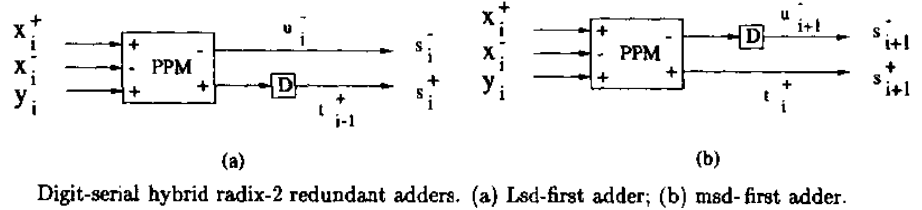
\includegraphics[width=0.8\textwidth]{figures/serial_mrHY4A.png}
                    \caption{Serial mrHY4A}
                    \label{fig:serial-mrHY4A}
                \end{figure}
            \end{center}
    \item   mr4 冗余表示不需要符号位,其所表示数字 $X$ 的符号蕴含在 
            $\{x_i^{-2},x_i^{+},x_i^{++}\}$ 的大小关系之中,这让我们避免了运算过程中的符号位扩展问题。
\end{itemize}

在浮点运算中,浮点加法的设计难度在于尾数的对齐。
因而相较于定点数加法,浮点数加法具有更高的硬件复杂度。
本文基于冗余mr4表示,针对浮点加法提出了一个大端先入的折叠计算模块。
如下图所示为量化精度为 $6$ 个数位($12$ 个二进制位)的冗余浮点加法运算过程,
为保持输出仍为6位的量化精度,该串行加法执行 $6$ 次,串行输出 $S=A+B$ 的每一个冗余数位。
其中,$B$ 的阶码比 $A$ 小3阶,故而在大端加法的前3个周期,只有数字 $A$ 所属移位寄存器移位输出。
在浮点数的串行加法中,大端先入是避免复杂对齐操作的关键,而冗余计算的大端先入串行加法具有和小端先入同等的复杂程度。
\begin{center}
    \begin{figure}[hb!]
        \centering
        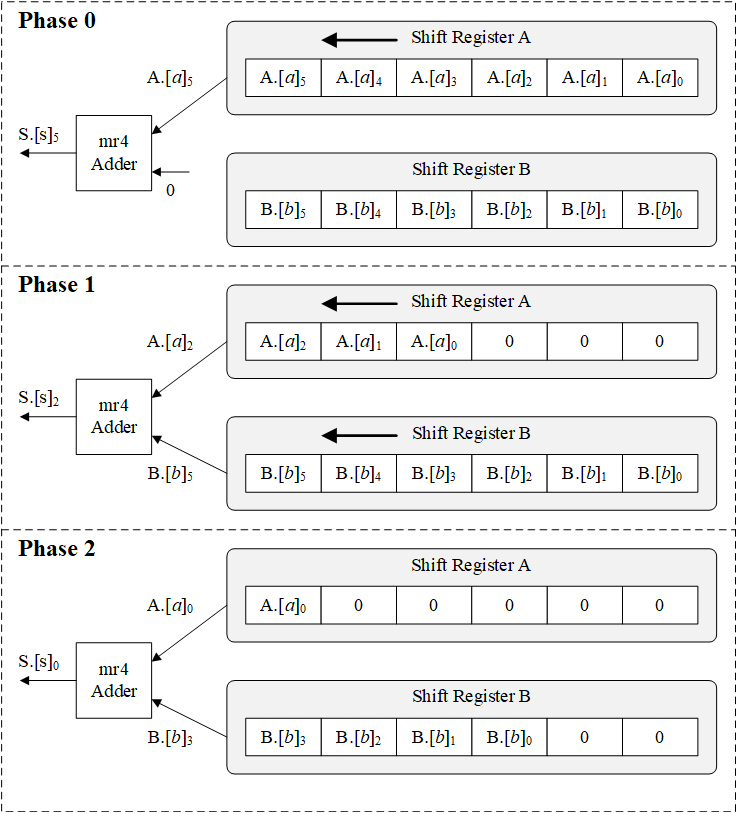
\includegraphics[width=0.55\textwidth]{figures/Float_Redundant_Adder.png}
        \caption{冗余浮点加法运算过程}
        \label{fig:Float-Redundant-Adder}
    \end{figure}
\end{center}

为配合大端先入的冗余浮点加法模块,本文继续设计了一款大端先入先出的串行冗余乘法单元,其主要电路结构入下图所示。
图中乘法器输入为FIR数据点 $X$ 和 FFT 单位根 $R$,其中在单次乘法过程中,$R$ 为固定输入,
而$X$ 所在的串行移位寄存器连接到 Booth 编码器(Booth Encoder)的输入端,完成对单位根 $R$ 的Booth编码,
编码输出作为当前输入与部分积 $D$ 累加。因为冗余加法不存在进位传播,故而 $D$ 的最高位 $D6$ 可以直接作为当前乘积的有效位而输出。
该结构迭代6次即可完成一次 $6$ 数位($12 \, \mathrm{bit}$ 精度)的乘法。
\begin{center}
    \begin{figure}[ht!]
        \centering
        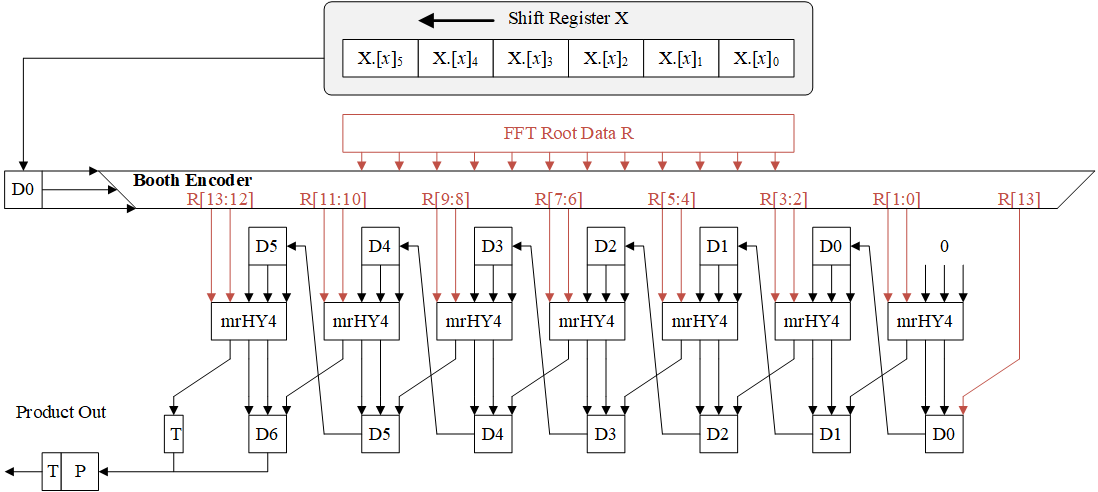
\includegraphics[width=0.6\textwidth]{figures/Redundant_Multiplier.png}
        \caption{冗余浮点乘法运算过程}
        \label{fig:Redundant-Multiplier}
    \end{figure}
\end{center}

\paragraph{\heiti{Karatsuba 快乘}}
以下对于高精度大整数乘法的 Karatsuba 算法简介摘录自 \href{https://oi-wiki.org/math/bignum/#karatsuba-%E4%B9%98%E6%B3%95}{OI Wiki:Karatsuba Algorithm}。

如果取高精度数字(必要时同时约化为大整数)的位数为 $n$,那么高精度—高精度竖式乘法需要花费 $\O(n^2)$ 的时间。
本节介绍一个时间复杂度更为优秀的算法,由前苏联(俄罗斯)数学家 Anatoly Karatsuba 提出,是一种分治算法。

考虑两个十进制大整数 $x$ 和 $y$,均包含 $n$ 个数码并可以有前导零。任取 $0 < m < n$,记
\begin{eqnarray*}
    \begin{aligned}
        x &= x_1 \cdot 10^m + x_0, \\
        y &= y_1 \cdot 10^m + y_0, \\
        x \cdot y &= z_2 \cdot 10^{2m} + z_1 \cdot 10^m + z_0,
    \end{aligned}
\end{eqnarray*}

其中 $x_0,y_0,z_0,z_1 < 10^m$。简单四则运算可得
\begin{eqnarray*}
    \begin{aligned}
        z_2 &= x_1 \cdot y_1, \\
        z_1 &= x_1 \cdot y_0 + x_0 \cdot y_1, \\
        z_0 &= x_0 \cdot y_0.
    \end{aligned}    
\end{eqnarray*}

继续观察(本质上使用分配律或 Wingoard 加速算法)将
\begin{eqnarray*}
    z_1 = (x_1 + x_0)(y_1 + y_0) - z_2 - z_0
\end{eqnarray*}

从而只要计算出 $(x_1+x_0), (y_1 + y_0)$ 再与 $z_2,z_0$ 相减即可求出 $z_1$。

因为普遍讲计算机上乘法的耗时要大于甚至远大于加法(尤其是数位越大的时候)。从而将乘法替换为
加法会大大降低算法的渐进时间复杂度。

上式实际上是 Karatsuba 算法的核心,它将长度为 $n$ 
的乘法问题转化为了 3 个长度更小的子问题。若令 
\begin{eqnarray*}
    m = \left\lceil \dfrac n 2 \right\rceil
\end{eqnarray*} 

记 Karatsuba 算法计算两个 $n$ 位整数乘法的耗时
为 $T(n)$,则有 
\begin{eqnarray*}
    T(n) = 3 \cdot T \left(\left\lceil \dfrac n 2 \right\rceil\right) + \O(n)
\end{eqnarray*}

由主定理可得 
\begin{eqnarray*}
    T(n) = \O (n^{\log_2 3}) \approx \O (n^{1.585})
\end{eqnarray*}

这相比于通常的大整数乘法的 $\O (n^2)$ 有数量级的减少。也回答了 20世纪 60年代 Kolmogorov 关于大整数乘法渐进时间复杂度是否
为 $\Omega(n^2) \approx \O (n^2)$ 的重大问题。

而 Anatoly Karatsuba 发明这个算法时年仅 23 岁,仅仅是在 Kolmogorov 陈述他关于任何大整数乘法算法的
时间复杂度趋于 $\O(n^2)$ 这一猜测一周后 Karatsuba 就完成了上述更快算法的构造。具体的历史信息可参考 
\href{https://en.wikipedia.org/wiki/Karatsuba_algorithm}{Wikipedia:Karatsuba Algorithm}。其中一段摘录如下

\begin{quote}
    In 1960, 
    Kolmogorov organized a seminar on mathematical problems in cybernetics 
    at the Moscow State University, where he stated the $\Omega (n^2)$ conjecture and other problems 
    in the complexity of computation. Within a week, Karatsuba, then a 23-year-old student, found an
     algorithm that multiplies two n-digit numbers in $\O (n^{\log_2 3})$ elementary steps, thus 
    disproving the conjecture. Kolmogorov was very excited about the discovery; 
    he communicated it at the next meeting of the seminar, which was then terminated. 
    Kolmogorov gave some lectures on the Karatsuba result at conferences all over the world 
    (see, for example, ``Proceedings of the International Congress of Mathematicians 1962'', 
    pp. 351–356, and also ``6 Lectures delivered at the International Congress of Mathematicians 
    in Stockholm, 1962'') and published the method in 1962, in the Proceedings of the USSR Academy 
    of Sciences. The article had been written by Kolmogorov and contained two results on 
    multiplication, Karatsuba's algorithm and a separate result by Yuri Ofman; it listed 
    \textquotedbl A. Karatsuba and Yu. Ofman\textquotedbl as the authors. Karatsuba only became aware of the paper 
    when he received the reprints from the publisher.
\end{quote}

更完整的第一手算法理论参考可见 Karatsuba 本人的综述 \cite{Karatsuba1995}。本项目使用其思想实现了针对滤波器乘法的版本如下,
主要集成了 Karatsuba 算法实现了多项式乘法和卷积,最后再处理所有的进位问题。具体信息参考源代码或附录。

\subsection{\heiti{量化感知中的混合精度量化(Mixed Precision Quantization)}}

此部分主要参考 \citetitle{Gholami2021} 的大量参考文献中实现的不同的量化感知技术。

\paragraph{\heiti{混合精度量化}}

选取最优的数据混合精度,硬件可以追求准确度与计算成本之间的平衡。

量化感知技术为硬件带来了效率提升。我们能够发现,在低精度计算模式下,量化感知技术可以让硬件计算速度完成提升。
但我们发现,对于一个元件而言,全部计算参数的低精度处理常常会带来元件工作准确度的大幅下降。
因此,为了保证元件工作的准确性,同时维持元件的高效运行,不同硬件采用不同的计算精度成为了合适的选择。
混合精度量化因此被提出,旨在研究对于某一固定硬件架构,应该选择什么样的低精度计算策略。

\begin{center}
    \begin{figure}[ht!]
        \centering
        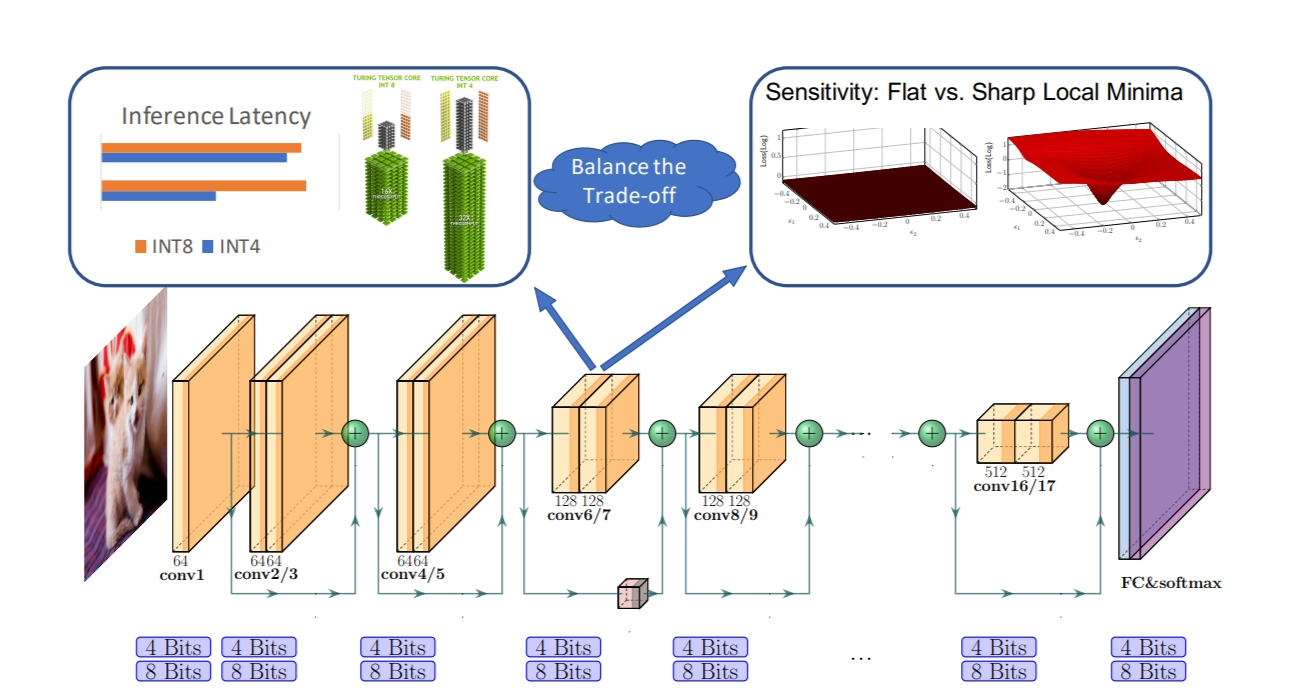
\includegraphics[scale = 0.5]{figures/multprecision.png}
        \caption{一种混合精度神经网络架构}
        \label{fig:multprecision}
    \end{figure}
\end{center}

如图\ref{fig:multprecision}所示,整个神经网络架构的各个卷积层分别选取了不同的参数精度,在不同参数精度的条件下分别进行训练。
在训练过程中挑选效果最优的精度组合,最终构成硬件结构的实际参数。

上述过程是混合精度量化的大体过程。对于混合精度量化模型的训练而言,通常有不同的训练方式。

在量化模型训练过程中,通常采用与全精度浮点模型不同的方式。如图\ref{fig:differentlpmethods}左表示的是浮点模型的训练方式。
浮点模型直接通过浮点数运算进行网络训练。而计算机在处理量化模型时一般采用模拟量化训练与完全量化训练两种方式,即图\ref{fig:differentlpmethods}剩余两部分的量化训练方法。


\begin{center}
    \begin{figure}[ht!]
        \centering
        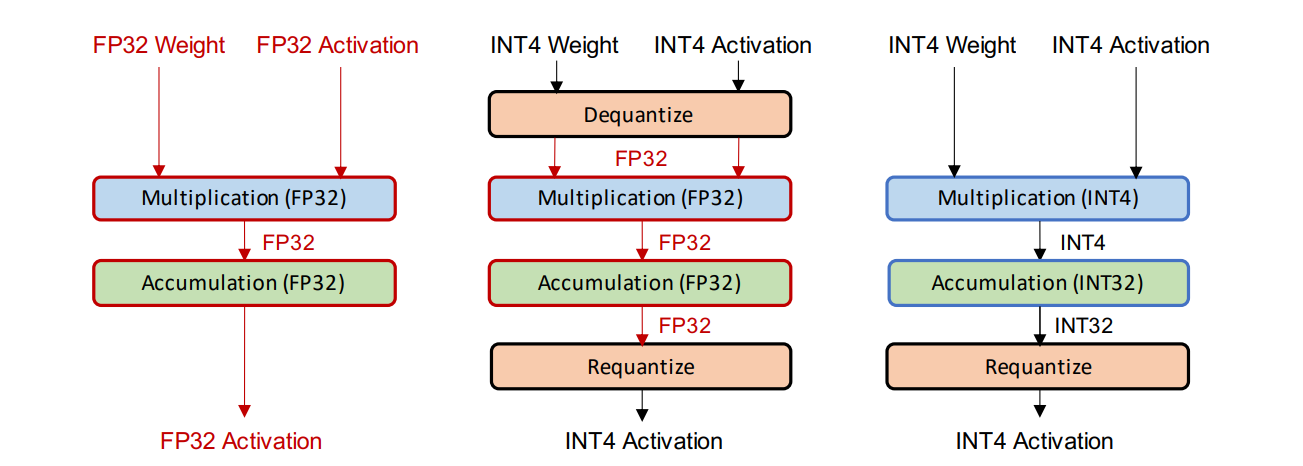
\includegraphics[scale = 0.5]{figures/differentLPmethods.png}
        \caption{量化神经网络的模型训练方法}
        \label{fig:differentlpmethods}
    \end{figure}
\end{center}


模拟训练量化的全部参数被储存在不同精度格式下,但在训练时首先通过计算将参数转化为浮点数,再利用浮点数的训练模式进行参数训练。
浮点数参数训练的优势在于其训练时非线性部分可以被有效近似,训练比较稳定。

完全训练量化则是根据低精度的数据格式的计算来进行模型训练。在低精度下,求导等运算的准确度会有所降低,可能会引入较大的计算误差。
因此,寻求更为有效的低精度近似计算方法是提高量化模型训练效率的重要方向之一。

上述两种量化训练方式各有优势与劣势,在不同的训练任务中需要根据侧重进行合适地选取。
量化感知的混合精度量化技术仍然具有提升潜力,更为有效的低精度计算方法将为混合量化模型的训练提供更加有效的提升。